\section{Core Innovations and Defensibility}
\label{sec:moat}

The programme's contribution is not a single steering trick but a coherent stack in which each layer is independently defensible and, taken together, hard to reconstruct from any one published component. This section states the core innovations explicitly and identifies what distinguishes them from the closest prior art.

\subsection{A Doctrine, Not a Vector}

The dominant mode in activation steering is to publish a direction and a layer. The innovation here is a doctrine that governs the direction: where to write in the band's own coordinates, when to write by online entropy, how to verify by band-targeted readback, and how much to spend against a registered freedom budget. Each clause is separately falsifiable and two failed in their first registered form (Sections~\ref{sec:results:timing} and~\ref{sec:results:moat}), which is the evidence that the clauses carry content rather than restating a convention. The measured ablations quantify what each clause buys: removing coordinate discipline collapses transfer lift from 0.40 to 0.05, removing timing costs roughly half the gated advantage, removing the budget quadruples the entropy cost, and using the final-target lens for verification misreads a loaded band as empty at subtle doses.

\subsection{Reading in the Band's Own Basis}

The second innovation is instrumental. Prior lenses read intermediate states toward the final output basis \cite{Nostalgebraist2020,Belrose2023}; this work reads and writes in the coordinates the workspace band itself articulates, through the transport transpose $J^{\top}u$. The head-to-head benchmark against the Jacobian-lens final-target baseline (Section~\ref{sec:results:baseline}) shows the practical payoff: at the subtle, budget-respecting doses where an intervention should operate, band-targeted reading is roughly twice as sensitive, with the direction decisive at $p=2.1\times10^{-5}$. The honest bound is equally part of the innovation: at saturating doses the instruments converge, so the claim is sensitivity at low dose, not universal invisibility.

\subsection{Recognition as a Deployable Defence}

The third and most consequential innovation is the recognition gate. The finding that a contrastive direction added unconditionally does not improve safety (Section~\ref{sec:results:alignment}) is, on its own, a negative shared with prior work. The advance is to use the same activation signal as a recognition test on the input rather than as a blanket write, and to show that this converts an unusable brute-force defence (which over-refuses every benign prompt) into one that matches the brute-force attack-success reduction at zero benign collateral on models whose benign and attack projections separate cleanly (Section~\ref{sec:results:moat}). Two properties make this a defensible moat rather than a demonstration. First, it operates at the activation level, so prompt-rewrapping attacks that defeat prompt-level filters do not evade it, consistent with the characterisation that these models are prompt-robust but activation-vulnerable. Second, and unusually for a safety intervention, its success is predictable before deployment from the same clean-gap statistic that drives it at inference time, so a deployer can determine offline and cheaply whether the defence will hold for a given model. The four-model result, works on two and predicted on all four, is presented as an existence-and-predictability claim under exploratory conditions, not a universal guarantee.

\subsection{A Reproducible Research Instrument}

The fourth innovation is methodological and is released as running software. The expected-free-energy selector over registered menus, closed by dual code-and-domain gates and audited by isolated adversarial reviewers, produced a programme in which every decision replays from committed artifacts and every reported number traces to a gate record. The audit trail did load-bearing work rather than decoration: it caught a sampling-stream correlation that re-based every early estimate, forced a formal supersession of stale dose levels, and withdrew a claimed replication that proved to be a determinism artifact. This instrument, together with the companion circuit-discovery agent \cite{Sathish2026ACD}, constitutes a template for small-compute interpretability research whose claims survive adversarial scrutiny.

\subsection{An Integrated, Released Product}

The innovations are not left as a paper. They ship as a Python package, fitted lens checkpoints for the studied models, a Model Context Protocol server and agent plugin that expose the lens-and-steer loop as callable tools, and interactive applications that render internal-state traces and replay the recognition-gated defence. Figure~\ref{fig:thought} shows the paper-static analogue of the interactive workspace view: a layer-by-token map of lens read-out grounded in the measured articulation gradient, annotated with a gated write and its band-targeted readback, in the spirit of the slice visualisation released with the workspace instrument \cite{Anthropic2026Workspace,JacobianLens2026}. The defensibility of the whole rests on the combination: the doctrine, the band-basis instrument, the predictable recognition gate, the audited research loop, and the released tooling reinforce one another, and reproducing the stack requires all of them rather than any single vector or lens.

\begin{figure}[t]
\centering
\resizebox{0.92\columnwidth}{!}{% Hand-authored TikZ. Workspace "thought" visualization in the style of the
% Jacobian-lens slice view: a layer x token grid whose cell shading is the
% lens read-out negentropy from gate L7 (band articulation), with an
% entropy-gated write event and its band-targeted readback annotated. This is
% the paper-static analogue of the interactive trace players in apps/web.
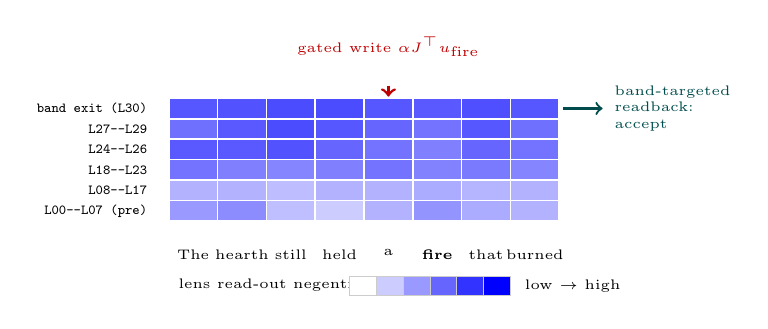
\begin{tikzpicture}[font=\scriptsize]
\def\cw{0.62}   % cell width
\def\ch{0.26}   % cell height
% negentropy by layer (gate L7 jacobian_lens.per_layer_negentropy, subsampled
% to the eight decode positions shown); higher = brighter band read-out.
% columns = decode tokens; rows = layer bands (early -> workspace band exit)
% each row is a layer group; shading value in [0,1] from the L7 array.
\foreach \r/\lab/\vals in {
  6/{band exit (L30)}/{0.66,0.68,0.70,0.70,0.66,0.65,0.69,0.66},
  5/{L27--L29}/{0.56,0.65,0.70,0.66,0.60,0.55,0.66,0.56},
  4/{L24--L26}/{0.65,0.65,0.68,0.60,0.55,0.50,0.60,0.55},
  3/{L18--L23}/{0.55,0.50,0.48,0.50,0.55,0.49,0.52,0.48},
  2/{L08--L17}/{0.30,0.30,0.26,0.30,0.30,0.33,0.29,0.30},
  1/{L00--L07 (pre)}/{0.40,0.45,0.25,0.20,0.30,0.42,0.33,0.30}}{
  \foreach \c/\v in {0/\vals} {}
  \pgfmathsetmacro{\y}{\r*\ch}
  \node[anchor=east, font=\tiny\ttfamily] at (-0.15,\y+0.5*\ch) {\lab};
  \foreach \c [count=\ci from 0] in \vals {
    \pgfmathsetmacro{\x}{\ci*\cw}
    \pgfmathsetmacro{\shade}{100*\c}
    \fill[blue!\shade!white, draw=white, line width=0.6pt]
      (\x,\y) rectangle (\x+\cw,\y+\ch);
  }
}
% token labels along the bottom (a representative gated fire-case decode)
\foreach \c/\tok [count=\ci from 0] in {0/The,1/hearth,2/still,3/held,4/a,5/{\bf fire},6/that,7/burned} {
  \pgfmathsetmacro{\x}{\ci*\cw + 0.5*\cw}
  \node[anchor=north, font=\tiny] at (\x,0.02) {\tok};
}
% write event (sphuratta gate) at the high-entropy step before "fire"
\draw[->, red!75!black, line width=1pt]
  (4.5*\cw,6*\ch+0.42) -- (4.5*\cw,6*\ch+\ch+0.02);
\node[red!75!black, font=\tiny, anchor=south] at (4.5*\cw,6*\ch+\ch+0.40)
  {gated write $\alpha J^{\top}u_{\mathrm{fire}}$};
% readback annotation at the band exit
\draw[->, teal!60!black, line width=0.8pt]
  (8*\cw+0.05,6*\ch+0.5*\ch) -- (8*\cw+0.55,6*\ch+0.5*\ch);
\node[teal!60!black, font=\tiny, anchor=west, align=left]
  at (8*\cw+0.58,6*\ch+0.5*\ch) {band-targeted\\readback:\\accept};
% colour key
\node[font=\tiny, anchor=west] at (0,-0.55) {lens read-out negentropy:};
\foreach \i in {0,...,5} {
  \pgfmathsetmacro{\sh}{20*\i}
  \pgfmathsetmacro{\x}{2.3+\i*0.34}
  \fill[blue!\sh!white, draw=gray!40] (\x,-0.68) rectangle (\x+0.34,-0.44);
}
\node[font=\tiny, anchor=west] at (4.4,-0.56) {low $\rightarrow$ high};
\end{tikzpicture}
}
\caption{Workspace read-out for a gated fire-case decode, the paper-static analogue of the interactive trace player in the released application. Cell shading is lens read-out negentropy by layer band and decode position, grounded in the measured articulation gradient (gate L7); the red arrow marks the entropy-gated write of the fire concept code at an uncommitted moment, and the readout at the band exit records the band-targeted acceptance verdict. This is the internal-state view that the doctrine reads and writes.}
\label{fig:thought}
\end{figure}